\chapter{Вхід в систему}

\section{Аутентифікація та авторизація}

Для входу в Систему:
--- під’єднайте ключ до USB порту;
--- інтерфейс екранної форми буде виглядати як зображено на Рисунку 3.1;

\begin{figure}[!htbp]
\centerline{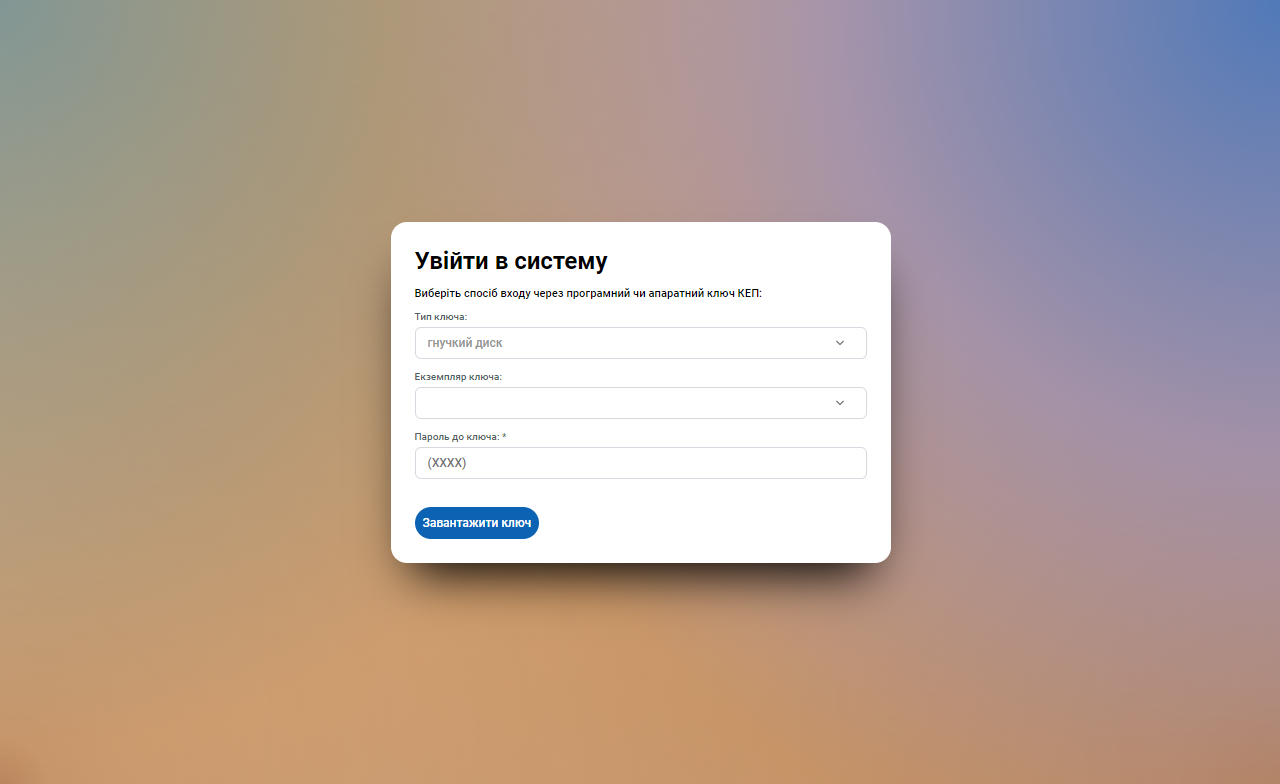
\includegraphics[width=\textwidth]{img/3.1.1.png}}
\caption{Вхід в систему}
\end{figure}

\newpage

--- введіть пароль до ключа $\rightarrow$ область введення даних, позначена цифрою 1 на Рисунку 3.1.2;
--- натисніть активний елемент «Завантажити ключ» → позначено цифрою 2 на Рисунку 3.1.2.

\begin{figure}[!htbp]
\centerline{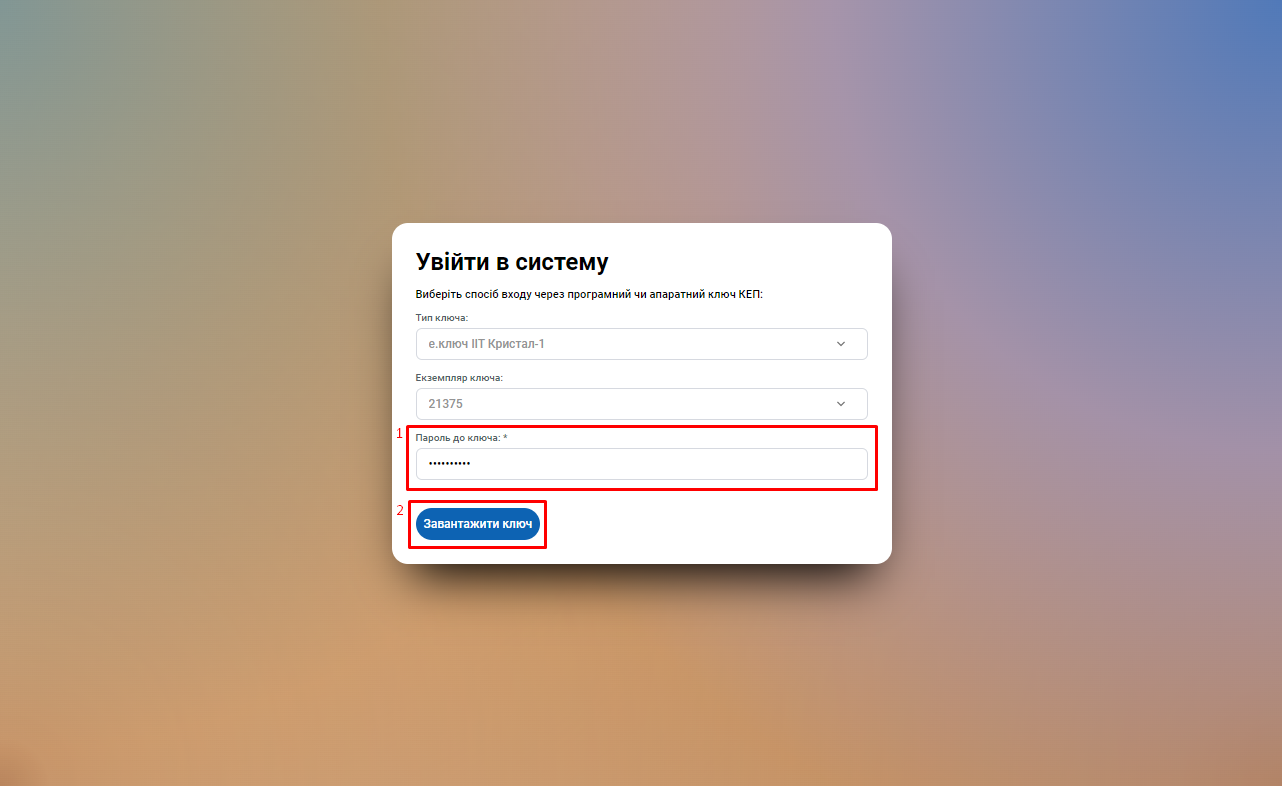
\includegraphics[width=\textwidth]{img/3.1.2.png}}
\caption{Пароль до ключа}
\end{figure}

--- у разі успішної авторизації Система завантажить Робочий стіл користувача (див. Рисунок 3.1.3)

\begin{figure}[!htbp]
\centerline{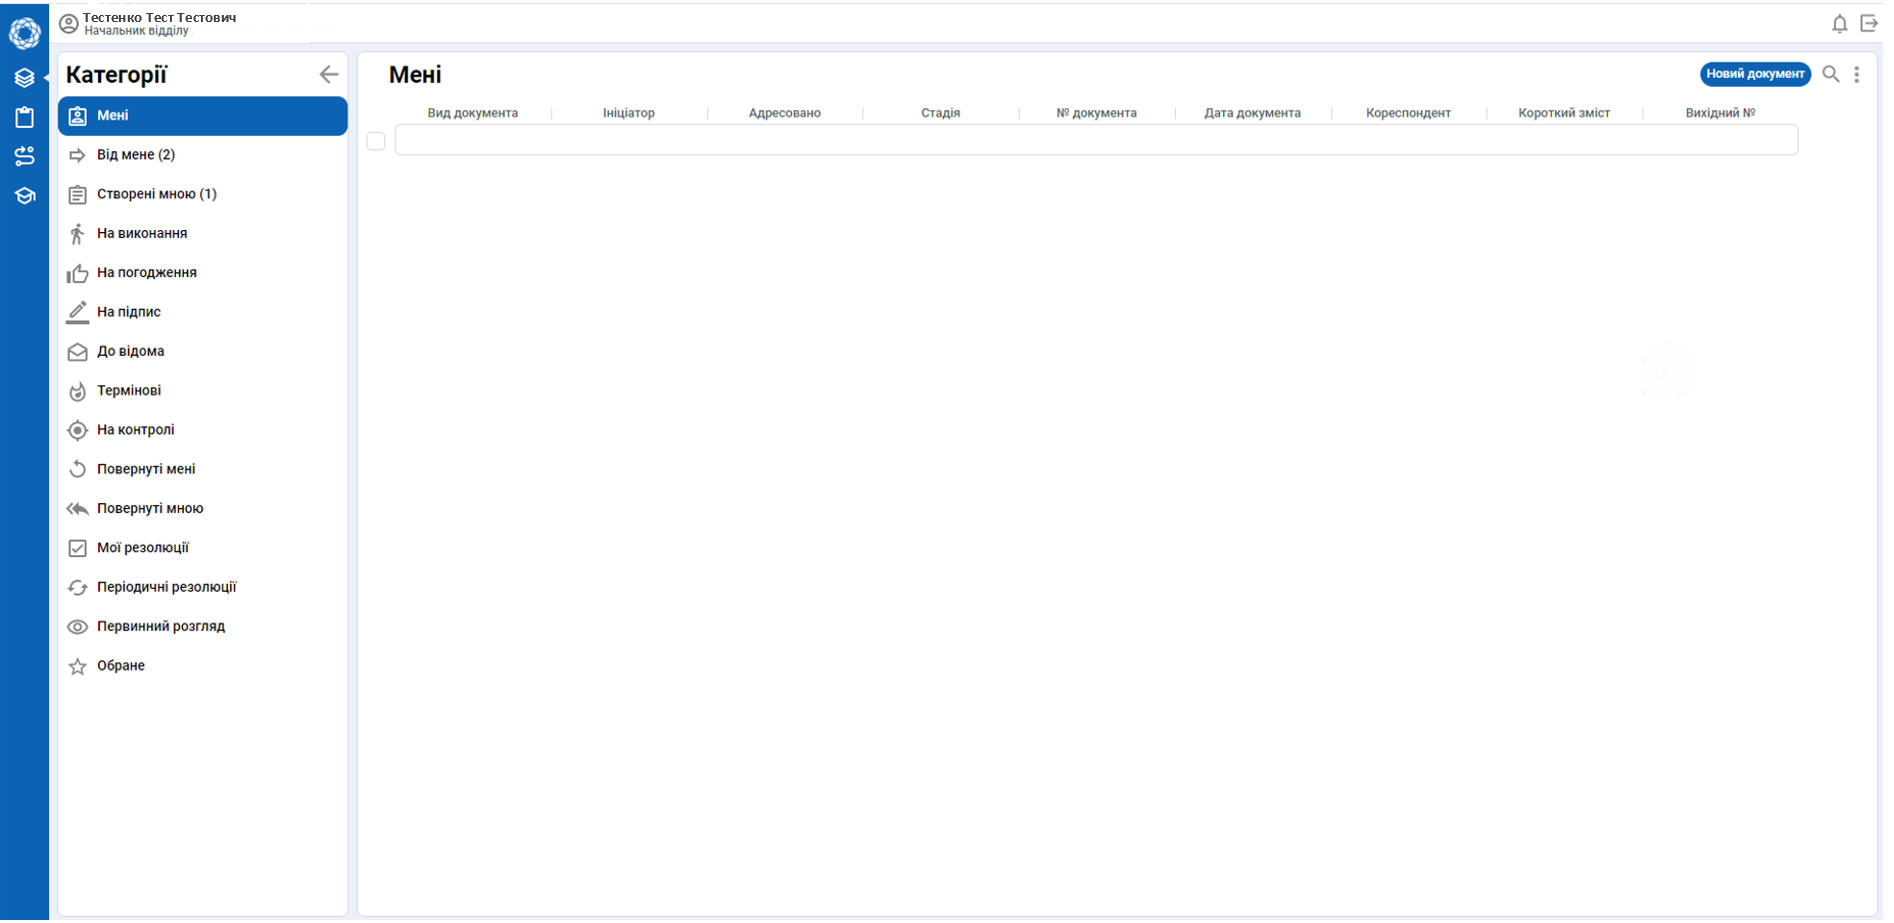
\includegraphics[width=\textwidth]{img/3.1.3.png}}
\caption{Робочий стіл користувача}
\end{figure}

